\documentclass[tikz,border=14pt]{standalone}
\usetikzlibrary{arrows.meta,positioning,shapes.geometric}
\begin{document}
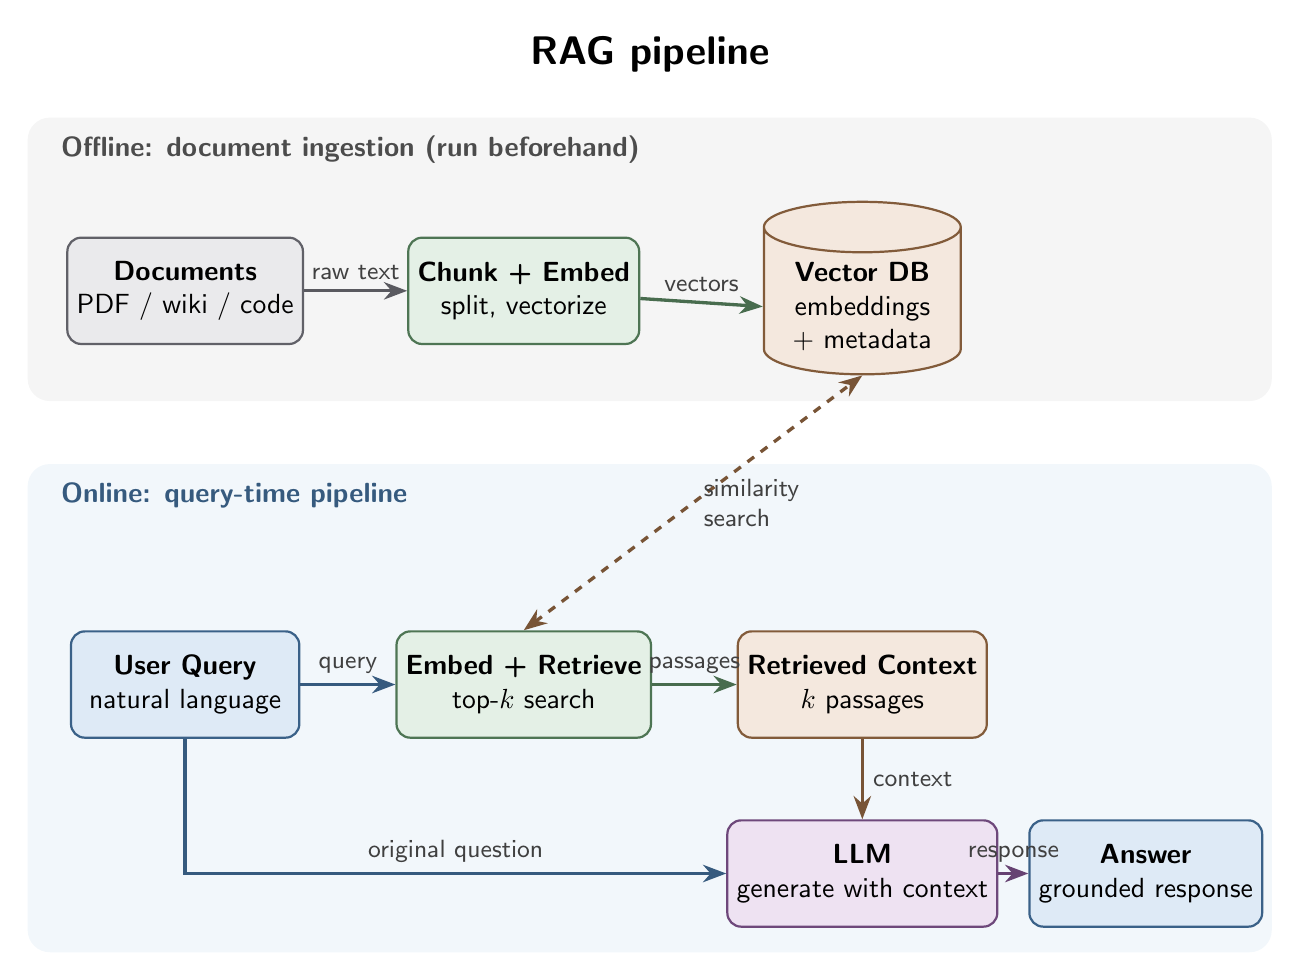
\begin{tikzpicture}[
  >=Stealth,
  font=\sffamily,
  box/.style={draw=#1!65!black,fill=#1!20,rounded corners=5pt,
    minimum width=2.9cm,minimum height=1.35cm,align=center,thick},
  db/.style={draw=#1!65!black,fill=#1!20,cylinder,shape border rotate=90,
    aspect=0.32,minimum width=2.5cm,minimum height=1.9cm,align=center,thick},
  flow/.style={->,very thick,#1!60!black},
  lab/.style={font=\small\sffamily,text=gray!50!black}]

  \definecolor{user}{RGB}{90,150,210}
  \definecolor{proc}{RGB}{120,180,130}
  \definecolor{store}{RGB}{200,140,90}
  \definecolor{llm}{RGB}{170,110,190}
  \definecolor{docz}{RGB}{150,150,160}

  % ---- lanes ----
  \fill[gray!8,rounded corners=8pt] (-2.0,3.0) rectangle (13.8,6.6);
  \node[font=\sffamily\bfseries,text=gray!60!black,anchor=west] at (-1.7,6.2)
    {Offline: document ingestion (run beforehand)};
  \fill[user!8,rounded corners=8pt] (-2.0,-4.0) rectangle (13.8,2.2);
  \node[font=\sffamily\bfseries,text=user!60!black,anchor=west] at (-1.7,1.8)
    {Online: query-time pipeline};

  % ---- offline row ----
  \node[box=docz] (docs) at (0,4.4) {\textbf{Documents}\\PDF / wiki / code};
  \node[box=proc] (chunk) at (4.3,4.4) {\textbf{Chunk + Embed}\\split, vectorize};
  \node[db=store] (vdb) at (8.6,4.2) {\textbf{Vector DB}\\embeddings\\+ metadata};

  \draw[flow=docz] (docs) -- (chunk) node[lab,midway,above] {raw text};
  \draw[flow=proc] (chunk) -- (vdb.west) node[lab,midway,above] {vectors};

  % ---- online row A: retrieval ----
  \node[box=user] (query) at (0,-0.6) {\textbf{User Query}\\natural language};
  \node[box=proc] (embed) at (4.3,-0.6) {\textbf{Embed + Retrieve}\\top-$k$ search};
  \node[box=store] (ctx) at (8.6,-0.6) {\textbf{Retrieved Context}\\$k$ passages};

  \draw[flow=user] (query) -- (embed) node[lab,midway,above] {query};
  \draw[flow=proc] (embed) -- (ctx) node[lab,midway,above] {passages};

  % ---- online row B: generation ----
  \node[box=llm] (gen) at (8.6,-3.0) {\textbf{LLM}\\generate with context};
  \node[box=user] (ans) at (12.2,-3.0) {\textbf{Answer}\\grounded response};

  \draw[flow=store] (ctx.south) -- (gen.north) node[lab,midway,right] {context};
  \draw[flow=user] (query.south) |- (gen.west)
    node[lab,pos=0.75,above] {original question};
  \draw[flow=llm] (gen) -- (ans) node[lab,midway,above] {response};

  % ---- cross-lane link: retrieval hits the vector DB ----
  \draw[flow=store,<->,dashed] (embed.north) -- (vdb.south)
    node[lab,midway,right,align=left] {similarity\\search};

  % title
  \node[font=\sffamily\bfseries\Large] at (5.9,7.4) {RAG pipeline};
\end{tikzpicture}
\end{document}
